\section{Обзор существующих решений}

\subsection{Метод сравнения текста}
Такие методы являются классическими для определения плагиата в обычном тексте, то есть не нацелены на программный код. Они заключаются в сравнении текстовых представлений программ на основе таких метрик, как:
\begin{itemize}[label*=---]
	\item расстояние Жаккара~\cite{Jaccard};
	\item расстояние Джаро -- Виклера~\cite{Jaro};
	\item расстояние Левенштейна~\cite{Lev};
	\item Колмогоровская сложность~\cite{Kolm}.
\end{itemize}

В отличие от обычного текста, программный код нельзя маскировать с помощью замены кириллицы на латиницу, допущения орфографический ошибок или использовать изменение регистра (исключая строковые переменные).

Методы, основанные на сравнении текстов находят только заимствования первого типа. Такую проверку легко обойти, например, переименовав переменные и добавив свои комментарии. Такие методы не поддерживают несколько языков программирования. 

Текстовые методы можно использовать для первоначальной оценки плагиата, так как они работают значительно быстрее, чем остальные~\cite{text}. Также, их можно применять при проверке небольших программных кодов, которые реализуют заведомо известный алгоритм. Потому что в таком случае единственный плагиат, который в нем можно найти -- особенность структурирования кода и название переменных. 

\subsection{Метод сравнения токенов}
Метод основан на преобразовании ключевых слов программы в токены -- последовательности лексических единиц с определенным значением~\cite{token}. 
\pagebreak
Токенизация осуществляется по следующему алгоритму.
\begin{enumerate}
	\item Каждому оператору языка программирования или группе операторов, имеющих схожее назначение, присваивается уникальный идентификатор. Значения идентификаторов назначаются заранее и для
	всех классов операторов.
	\item По полученным идентификаторам строится строка. В данной строке порядок токенов соответствует порядку следования их в исходном коде.
	\item Полученные токены сравниваются любым доступным способом
\end{enumerate}

Такой подход находит плагиат первых двух типов, также он может выявлять заимствованные фрагменты кода, которые расположены в различных местах программы, но делает это с неточностями. Поддержка разных языков программирования возможна только при использовании нескольких лексических анализаторов.

Методы, использующие токены, как и текстовые методы можно использовать для первоначальной проверки плагиата. Также если все программные коды, которые необходимо проверить на плагиат написаны на одном языке программирования и реализуют одинаковый функционал, то такой подход дает хорошую точность.

\subsection{Метод сравнения метрик}
Метод дополняет алгоритмы токенизации~\cite{metric}. Помимо сравнения токенов он на их основе определяет метрики, например:
\begin{itemize}[label*=---]
	\item количество условных конструкций;
	\item количество используемых циклов;
	\item количество глобальных переменных. 
\end{itemize}

Также, зная специфику действий пользователей, можно выдвигать свои метрики, например -- учитывать время обновления кода или  количество пройденных с первого раза тестов, если они имеются.

На основе таких метрик высчитывается схожесть программных кодов. Такие методы достаточно легко обмануть, изменив структуру программы, например добавив лишние функции или пустые циклы. Все остальные характеристики аналогичны методу, использующему токены. 

\subsection{Метод сравнения деревьев}
Подход  основан на представлении кода в виде абстрактного синтаксического дерева. 

Абстрактное синтаксическое дерево (англ. \textit{Abstract Syntax Tree}) --  конечное помеченное ориентированное дерево, в котором внутренние вершины сопоставлены с операторами языка программирования, а листья -- с соответствующими операндами, то есть переменными и константами.

На рисунке \ref{img:ast}  изображено дерево для выражения while (x > 0) x = x - 1.
\begin{figure}[!h]
	\centering
	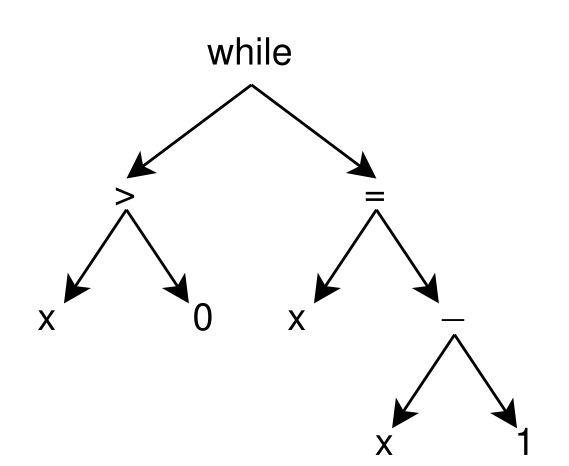
\includegraphics[width=100mm]{img/ast2}
	\captionsetup{justification=centering}
	\centering\caption{Представление структуры исходного кода в виде дерева}
	\label{img:ast}
\end{figure}

В таком формате программные коды сравниваются любым доступным способом. Таким образом, методы, основанные на абстрактных синтаксических деревьях состоят из двух этапов: построение деревьев и их анализ. Из наиболее популярных алгоритмов сравнения -- алгоритм Zhang-Shasha, который позволяет вычислять редакционное расстояние между деревьями~\cite{zhang}, или сравнение деревьев с помощью строковых ядер~\cite{kernel}.Таким образом можно выявить плагиат первых трех типов и осуществить поддержку нескольких языков программирования. 

\subsection{Метод низкоуровневого сравнения кода}

Данный метод сравнивает код после этапа компиляции или интерпретации~\cite{binary}. В зависимости от специфики языка программирования, такой подход может показывать разную точность. При этом заимствования первых двух типов наблюдается высокая точность, так как компилятор часто оптимизирует мелкие структурные изменения, например, замена for на while и наоборот в си-подобных языках программирования. Также такой метод дает хороший результат при модификациях третьего и четвертого типа, но его также можно легко понизить, например, поменяв типы данных (хранить числа в строковом представлении).

Такой подход можно успешно использовать, когда все программы компилируются одинаково и  имеют заведомо оговоренные типы данных. В таком случае можно определить заимствования всех типов.
